\chapter{Contexte général du projet}
\epigraph{SpaceX is a flat organization. Anyone gets to talk to anyone, and the best idea wins - even if it comes from an intern.}{Gwynne Shotwell}	
\subparagraph{}
Ce chapitre contextualise le projet dans son environment, en présentant en premier lieu l'organisme hôte de celui-ci – L'Office Chérifien des Phosphates – avant de motiver les raisons inhérentes à son implémentation pour finir sur la planification du déroulement de l'analyse, la conception et la réalisation du projet.
\cleardoublepage

\section{Présentation de l’OCP}
	\subsection{Historique}
	En 1920, alors que partout dans le monde, les compagnies minières fouillent fébrilement le
sous-sol à la recherche du phosphate, minerai aux précieuses vertus fertilisantes, l’Office
Chérifien des Phosphates (OCP S.A. depuis 2008) voit le jour.

En 1965, avec la mise en service du Maroc Chimie à Safi, le groupe devient également
exportateur de produits dérivés. En 1998, il franchit une nouvelle étape en lançant la fabrication
et l’exportation d’acide phosphorique purifié.

Parallèlement, de nombreux partenariats sont développés avec des opérateurs industriels du
secteur, au Maroc et à l’étranger.
	\subsection{Fiche signalétique}
	\begin{description}[align=left]
		\item [Nomination sociale :] Groupe Office Chérifien des Phosphates
		\item [Date de création :] 1920
		\item [Siège social :] 2-4, rue Al Abtal, Hay Erraha, 20200 Casablanca
		\item [Capital social :] 8287 M MAD (2013)
		\item [Effectif employé :] 23,000 (2013)
		\item [Site web :] www.ocpgroup.ma
	\end{description}
	\subsection{Chronologie des événements marquants de l’histoire du Groupe OCP.}
	\begin{description}[align=left]
		\item [1920 :] Création, le 7 août, de l'office chérifien des Phosphates (OCP).
		\item [1959 :] Création de la société marocaine d'études spécialisées et industrielles (SMESI).
		\item [1965 :] Création de la société Maroc Chimie.
		\item [1974 :] Lancement des travaux pour la réalisation du centre minier de Benguérir, en mai.
		\item [1975 :] Création du Groupe OCP avec l'intégration des industries chimiques aux
		\item [1998 :] Le Groupe OCP obtient le Prix National de la Qualité.
		\item [2003 :] L'OCP est devenu le seul actionnaire de Phosboucraâ.
		\item [2008 :] La société anonyme OCP SA est née le 22 janvier - Démarrage de Pakistan Maroc
		\item [2009 :] Démarrage de Bunge Maroc Phosphore à Jorf Lasfar (BMP).
		\item [2010 :] Création de JESA, joint-venture sous forme de partenariat en ingénierie
		\item [2012 :] Creation de la JV BSFT (Black Sea Fertilizer Trading Company)
		\item [2013 :] Signature d’une joint-venture avec Dupont
		\item [2014 :] Inauguration du SLURRY PIPELINE entre Khouribga et Jorf Lasfar
	\end{description}
	
	\subsection{Filiales et partenariats}
	L'OCP se structure en quatre filières chacune se focalisant sur un segment du groupe OCP et ayant co-créé plusieurs coentreprises. Ces partenariats ont été établis avec des clients du Groupe OCP. Ceci est le fruit d’une coopération qui touche aussi bien les accords de livraison à moyen et long terme que la
	construction d'unités de production. Dans cette optique, des unités basées au Maroc et à
	l'étranger sont en exploitation en joint-venture avec plusieurs partenaires dont la figure \ref{fig:mesh1} fait la liste : 
	\begin{figure}[h]
    		\centering
    		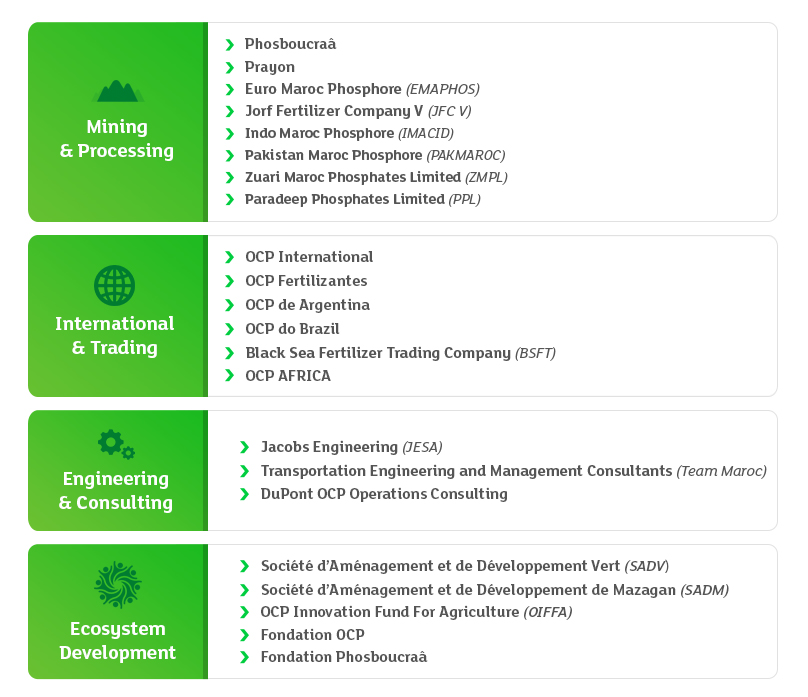
\includegraphics[scale=0.62]{Companies-ocp}
    		\caption{Filiales et coentreprises de l’OCP \cite{ocp-fil}}
    		\label{fig:mesh1}
	\end{figure}
	\subsection{Les principales activités du Groupe OCP}
	Les phosphates marocains sont exploités dans le cadre d'un monopole d'État confié à l'OCP.
	Le Groupe OCP a pour mission l'extraction, la valorisation et la commercialisation de
	phosphate et de ses produits dérivés. Chaque année, plus de 24 millions de tonnes de minerais
	sont extraites du sous-sol marocain qui recèle les trois quarts des réserves mondiales\footnote{Connue à ce jour (rapport US Geological Survey, 2011)}. Le phosphate brut provient des sites de Khouribga, Benguérir, Youssoufia et Boucraâ-Laâyoune. Généralement, le minerai subit une ou plusieurs opérations de traitement (criblage,séchage, calcination, flottation, enrichissement à sec ...). Celui-ci est ensuite exporté à l'état brut soit livré aux industries chimiques du groupe (à Jorf Lasfar ou à Safi) pour être transformé en produits dérivés commercialisables : acide phosphorique de base, acide phosphorique purifié et autres engrais solides, une large gamme de produits répondant à différents besoins, lui permettant de diversifier son portefeuille de clients
	et de faire face aux évolutions du marché \cite{NACER}.
		\par
		\textit{\textbf{Minerai de phosphate}}
		\par
		OCP est le premier exportateur mondial de phosphate brut avec 33 \% de parts de marché.
		\par
		\textit{\textbf{Acide phosphorique}} \par
		Produit intermédiaire entre le minerai et les engrais, l’acide phosphorique est en fait le fruit
		d’un enrichissement de la roche obtenu par réaction avec un ensemble d’acides différents à
		concentrations distinctes. L’acide phosphorique purifié est produit en moindres quantités destinées à des applications alimentaires et industrielles.\par OCP est le premier exportateur mondial d’acide phosphorique avec 46 \% de parts de marché.
		\par
			\textit{\textbf{Engrais phosphatés}} \par
		\begin{itemize}
		\item Le MAP est un engrais binaire composé de deux éléments fertilisants : le phosphore et l’azote.
		\item Le DAP est un engrais tertiaire composé de deux éléments fertilisants : le phosphore et l’azote, engrais le plus répandu.
		\item Le TSP est un engrais entièrement phosphaté.
		\item Le NPK est un engrais ternaire composé de trois éléments : phosphore, azote et potassium.
		\end{itemize}
		\paragraph{}
		L’influence du Groupe OCP vient de l’exportation de plus de 95\% de sa production en dehors
		des frontières nationales. Opérateur international, il est présent sur les cinq continents. Il occupe
		une place très importante dans l'économie nationale puisque ses exportations ont totalisé plus
		que 20\% des exportations marocaines. Il a ainsi contribué en 2013 à environ 4,3\% du PIB \cite{CHEMLAL}.
		\subsection{Organisation du groupe OCP}
		\subsubsection{Organigramme institutionnel}
		Présidé par le directeur général, le comité de direction exécutif compte sept directeurs exécutifs.
		Ils sont respectivement en charge de la direction du capital humain, du pôle industriel axe nord,
		du pôle industriel axe centre, du pôle commercial, du pôle finances et contrôle de gestion, du
		pôle stratégie \& corporate development\footnote{Developpement entreprise} et enfin du pôle juridique.
		\begin{figure}[H]
		    		\centering
		    		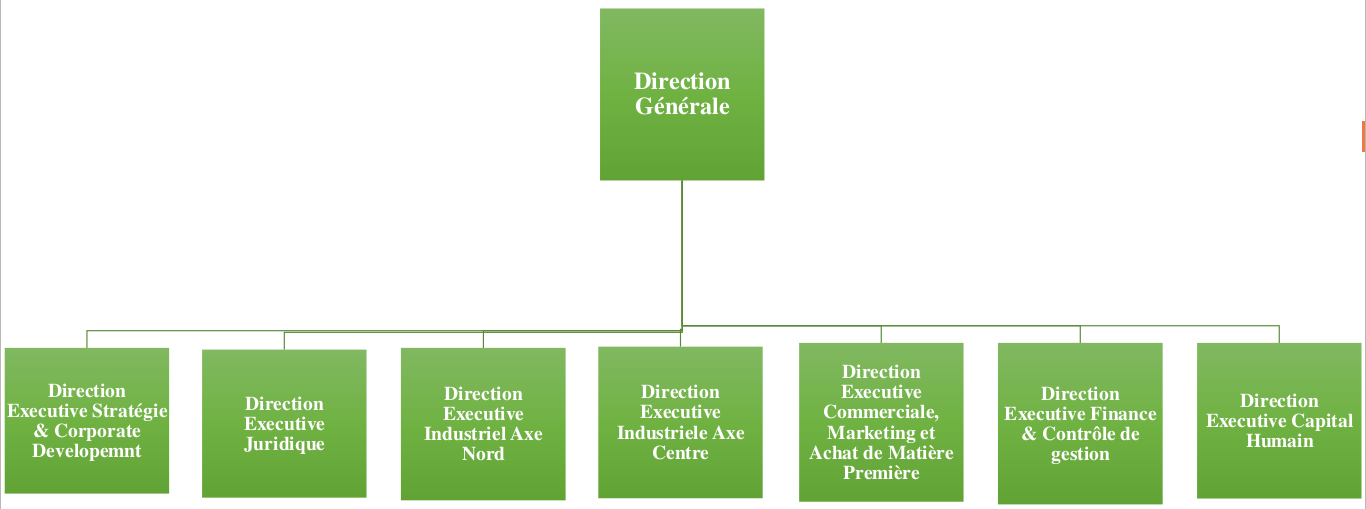
\includegraphics[scale=0.35]{Orga}
		    		\caption{Le management senior de l'OCP \cite{ocp-fil}}
		    		\label{fig:Orga}
			\end{figure}
		\subsubsection{La direction Commerciale-Marketing: hôte de notre stage}
		La direction commerciale, où nous avons effectué notre stage, joue un rôle central dans le dispositif mis
		en avant par la nouvelle stratégie de l'OCP. Elle est composée de six directions : direction des
		ventes (découpée en quatre régions), direction des opérations, direction marketing, direction
		logistique et maritime, direction "Business Developement"\footnote{Developpement des affaires} et la direction "Procurement"\footnote{Achat de matières
		premières}.
\section{Présentation du projet}
	\subsection{Définitions et terminologie}
	Avant de procéder plus en avant, il est nécessaire de définir certains termes couramment utilisés, mais ne possédant pas la même signification pour tout le monde. Dans la pratique, des termes comme «potentiel», «marché», «demande», et «ventes», sont utilisés de façon interchangeable. Aux besois du présent rapport, nous allons en premier lieu définir ces termes pour nous assurer de la clarté de leurs utilisations ci-après.
	\paragraph*{}
	Le terme «potentiel»  réfère à la quantité d'engrais qu'un pays ou une région de pays peut consommer dans des conditions optimales. L'ensemble de la superficie cultivée dans diverses cultures, multiplié par la dose d'engrais recommandée pour chaque culture est assimilable à la consommation d'engrais potentiel pour un pays.\par
	Il est évident que l'intérêt pour un engrais ou la possibilité de l'utiliser ne suffit pas d'elle-même pour expliquer la consommation. Les agriculteurs doivent d'abord avoir la conviction que par l'utilisation d'engrais, ils peuvent augmenter leurs revenus. Même si tel est le cas, ceux-ci ne seront pas forcément en mesure d'acheter des engrais. Cela dépend des liquidés financières dont ils disposent lors du besoin de l'engrais.\par
	Les agriculteurs s'attendent à ce que l'engrais dont ils ont besoin soit disponible en temps opportun. «L'accès» fait référence à la capacité du réseau de distribution de rendre le bon type d'engrais à disposition de l'agriculteur dans le temps et aussi facilement que possible. En fonction de ces facteurs, il existe un «marché» disponibles ou «demande». \textbf{La prévision de la demande est la quantité d'engrais susceptible d'être vendue sur une certaine période définie pour tout un pays ou region de pays.} Les termes «marché» et «demande» sont utilisés de manière interchangeable. Alors que le «marché» ou «demande» se réfèrent aux ventes de toutes les entreprises dans le pays, le terme «ventes» fait référence à une seule entreprise. Les ventes d'engrais d'une entreprise dépend ainsi de sa part de marché.
	\paragraph{}
	Les prévisions à court et à long terme servent à des fins différentes. Les prévisions à court terme sont concernées par la prochaine saison ou année. Les projections à court terme sont nécessaires pour organiser la production, l'approvisionnement en matériaux brutes, finis et d'emballage, le stockage, le transport et les fonds de roulement de sorte que la demande prévue est assurée avec succès. Les projections à long terme de plus de quatre à cinq ans sont utilisés pour les décisions de politique et d'investissement. L'investissement dans de nouvelles installations de production et de recherche, la formulation des plans de développement, le renforcement de l'établissement de crédit, etc., sont des exemples de décisions régies par les prévisions à long terme.
	\subsection{Cadre général du projet}
	L'OCP a itérativement modernisé ces processus d'organisation et de management dans la portée de promouvoir sa productivité et assurer le développement et la croissance continue
	par rapport à la concurrence. Une modernisation qui ne peut se passer d'un accompagnement informationel performant.\par
	De grandes avancées sont à noter, principalement dans le domaine de la Business Intelligence. Ceci a débuté par l’informatisation de ces procédés pour garantir une optimisation au niveau des durées de traitements que subit l’information et les fiabiliser. D'abord par la mise en place d’un portail décisionnel, à base de fichiers PDF dédié à la direction commerciale avant de se poursuivre en l’optimisation du temps d’accès à travers l’automatisation des processus de gestion de données, de
	réception des mails et extraction de données, mais aussi par le type des rapports (paramétrables
	interactifs, structures de coût) et leur publication dans un portail Web dédié.
	\par
	Ces données proviennent des organismes indépendants spécialisés dans l'analyse de marché. Hebdomadairement, la direction commerciale reçoit plus de 100 publications de ces organismes qui contiennent des guides de prix, des évaluations ou même des prévisions concernant le marché de phosphates, ses dérivées et les matières premières.
	\paragraph{}
	Durant notre familiarisation préliminaire avec l'existant, nous avons relevé plusieurs discrépances entre cet idéal informationnel voulu et la réalisation sur le terrain de cette vision, que nous détaillerons dans le second chapitre de ce rapport.
	\subsection{Motivation et problématique}
	\subsubsection{Motivation}
	Parce que la demande d'engrais dépend d'une variété de facteurs agro-économiques, celle-ci n’est pas stable, ni est-elle sujette à des prédictions exactes. Le choix des méthodes de prévision est donc particulièrement important, tant pour la gestion efficiente des compagnies productrices des engrais que pour la formulation de politiques appropriées par les gouvernements.
	La prévision efficace de la demande peut permettre aux exportateurs de tirer pleinement parti des fluctuations des cours mondiaux du marché. Le stockage requis, le transport, les ressources humaines à mobiliser, les arrangements financiers de crédits et de devises étrangères sont tributaires de la demande.
	\paragraph{}
	Considérant que les engrais produits mais non vendus peuvent être conservés pendant un an avant de trouver un acheteur et qu'une durée de stockage d'une année peut causer des partes en quantité et en qualité conséquentes, l'importance de la prévision de la demande peut être facilement appréciée. Si la demande réelle est plus grande que prévue, ce ci conduit à des pénuries, une production agricole inférieure et, souvent, à des implications politiques pour les pays importateurs.
	\paragraph{}
	Tous les plans des entreprises fabriquant ou commercialisant des engrais devraient être dérivés directement ou indirectement de la prévision de la demande. A partir d'une prévision internationale de la demande, les ventes attendues d'une entreprise peuvent être estimées en évaluant sa part de marché dans chaque région du pays.
	\par
	La prévision des ventes servira de consigne à l’égard du département de production quant à quoi, quand et combien produire. Le département financier de l'OCP, lui, est ainsi en mesure de préparer, sur la base des prévisions de ventes, un plan d'entrées et sorties de fonds, évaluer l'écart entre les fonds de roulement et d'organiser le soutien nécessaire de la banque. Le département marketing est guidé par la prévision dans le déploiement du personnel de vente, alors que le logistique sera éclairé quant à l’organisation du stockage à des endroits appropriés, les contrats de transport de marchandises pour faire face au volume prévu de l'entreprise.
	\subsubsection{Problématique}
	
	\paragraph{}
Au fil des années, la direction commerciale-marketing où nous avons effectué notre stage de fin d'études, a itérativement modernisé ses outils de traitement d'information. Dernière contribution en date de l'ENSIAS\footnote{Ecole Nationale Supérieure d'Informatique et d'Analyse des Systèmes - Grande Ecole d'Ingénieurs, Maroc} à cet essort informationnel, celle de Mr NACER \cite{NACER}, a consisté en la mise en place d'une solution adéquate basée sur les concepts et technologies du BI\footnote{Business Intelligence} ayant permis l'automatisation de la reception, de la normatisation et l'exploitation de tableau de bord post-analyse des données recuillies. Celle-ci se définissant comme une complétion du travail précurseur de Mr CHEMLAL \cite{CHEMLAL}.  La plateforme ainsi réalisée par nos prédecesseurs est ainsi un socle pour aider les décionnaires CM\footnote{Commercial-Marketing} à mieux appréhender les évolution et historiques des marchés mondiaux.
\paragraph{}Nous proposons d'emmener les perspectives informationelles du département CM au-delà du reporting \footnote{Tableaux de bord et rapports Business Intelligence} continu vers des mécanismes décisionnels et prévisionnels mettant en œuvre les techniques à l'état de l'art de fouilles de données (cf def data mining) . Nous souhaitons ainsi 'miner' des relations interessantes régissant le marché international des phosphates qui ne sauraient être mises en relief par les techniques de la BI à savoir la segmentation en faits, dimensions et mesures. Notre problématique s'articule ainsi:\subparagraph*{}\textbf{Quelles mécanismes prévisionnels peuvent être établis à la suite d'une recherche de structure précedemment inconnue dans le marché international des phosphates ?}\subparagraph*{}Répondre d'une manière exhaustive à cette question constituerait un atout clé en faveur d'une meilleure compétitivité de l'OCP et nous nous proposons d'explorer divers piste dont le présent rapport témoigne. 
\section{Planification du projet}
	\subsection{Les étapes CRISP-DM d'un projet Data Mining}
	CRISP-DM, qui signifie Cross-Industry Standard Process for Data Mining\footnote{Standard inter-entreprises du processus de fouille de données.}, est un modèle de processus d'exploration de données qui décrit les approches couramment utilisées par les experts pour résoudre des problèmes d'exploration de données \cite{CRISP-DM}.\par 
	Des sondages effectués en 2002, 2004, 2007 et 2014 montrent qu'il s'agit de la méthode principale utilisée par les data miners \cite{KDN}.\par
	
	CRISP-DM découpe le processus de data mining en six phases principales. La séquence des phases n'est pas stricte et un va et vient entre les différentes phases est toujours nécessaire. Les flèches dans le diagramme du processus indiquent les dépendances les plus importantes et fréquentes entre les phases. Le cercle extérieur dans le diagramme symbolise la nature cyclique de l'exploration de données. Un projet de fouille de données se poursuit après qu'une solution ait été déployée. Les leçons apprises au cours du processus peuvent déclencher de nouvelles questions métier, souvent plus ciblées et font bénéficier les processus d'extraction de données ultérieures de l'expérience des précédents. Les six phases sont résumés dans la figure \ref{fig:crisp}.
	\newpage
	\paragraph{Compréhension du problème:}
	Cette première phase se concentre sur la compréhension des objectifs et des exigences du projet à partir d'un point de vue commercial, puis convertir ces connaissances en une définition de problème d'extraction de données, et un plan préliminaire conçu pour atteindre les objectifs désirés.
	\paragraph{Compréhension des données:}
	La phase de compréhension des données commence par une collecte de données initiale et procède à des activités dans le but de se familiariser avec les données, pour identifier les problèmes de qualité des données, pour découvrir un premier aperçu de celles-ci, ou pour détecter des sous-ensembles intéressants pour former des hypothèses pour des informations cachées.
	\paragraph{Préparation des données:}
	\begin{wrapfigure}{r}{6.5cm}
	\raggedleft
	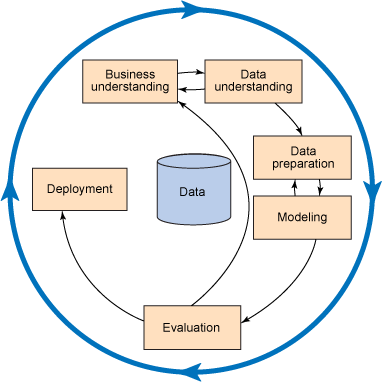
\includegraphics[scale=0.5]{crisp-dm}
	\caption{Les six phases de la méthodologie CRISP-DM}
	\label{fig:crisp}
	\end{wrapfigure}
	La phase de préparation des données couvre toutes les activités pour construire l'ensemble de données final (celui qui sera fourni en entrée aux algorithmes de modélisation) à partir des données brutes initiales. Cette tâche est susceptible d'être effectuée plusieurs fois, et pas dans un ordre prescrit. Celle-ci comprend la sélection des tables, des enregistrements, et des attributs d'interêt ainsi que leur transformation et nettoyage.
	\paragraph{Modélisation des Données:}
	Dans cette phase, les différentes techniques de modélisation sont choisies et appliquées, leurs paramètres sont étalonnés à des valeurs optimales. En règle générale, il existe plusieurs techniques pour le même type de problème d'exploration de données. Certaines techniques ont des exigences spécifiques sur la forme de données. Par conséquent, un retour à la phase de préparation des données est souvent nécessaire.
	\paragraph{Évaluation:}
	A ce stade du projet, un modèle qui semble avoir de bonnes propriétés, du point de vue de l'analyse des données a été construit. Avant de procéder au déploiement final du modèle, il est important d'évaluer de manière plus approfondie le modèle, et d'examiner les étapes exécutées pour la construction de celui-ci, pour être certain qu'il répond correctement aux objectifs métiers précédemment arrêtés.
	\paragraph{Déploiement:}
	La création du modèle est généralement pas la fin du projet. Même si le but est d'accroître les connaissances des données, l'acquis doit être organisé et présenté d'une manière qui est utile pour le commanditaire. Selon les besoins, la phase de déploiement peut être une simple génération de rapport aussi bien qu'une mise en œuvre de mécanismes prévisionnels.
	

	\begin{landscape}
	\subsection{Le planning du projet}
	\subsubsection{Diagramme de GANTT}
		\begin{figure}[H]
    			\centering
    			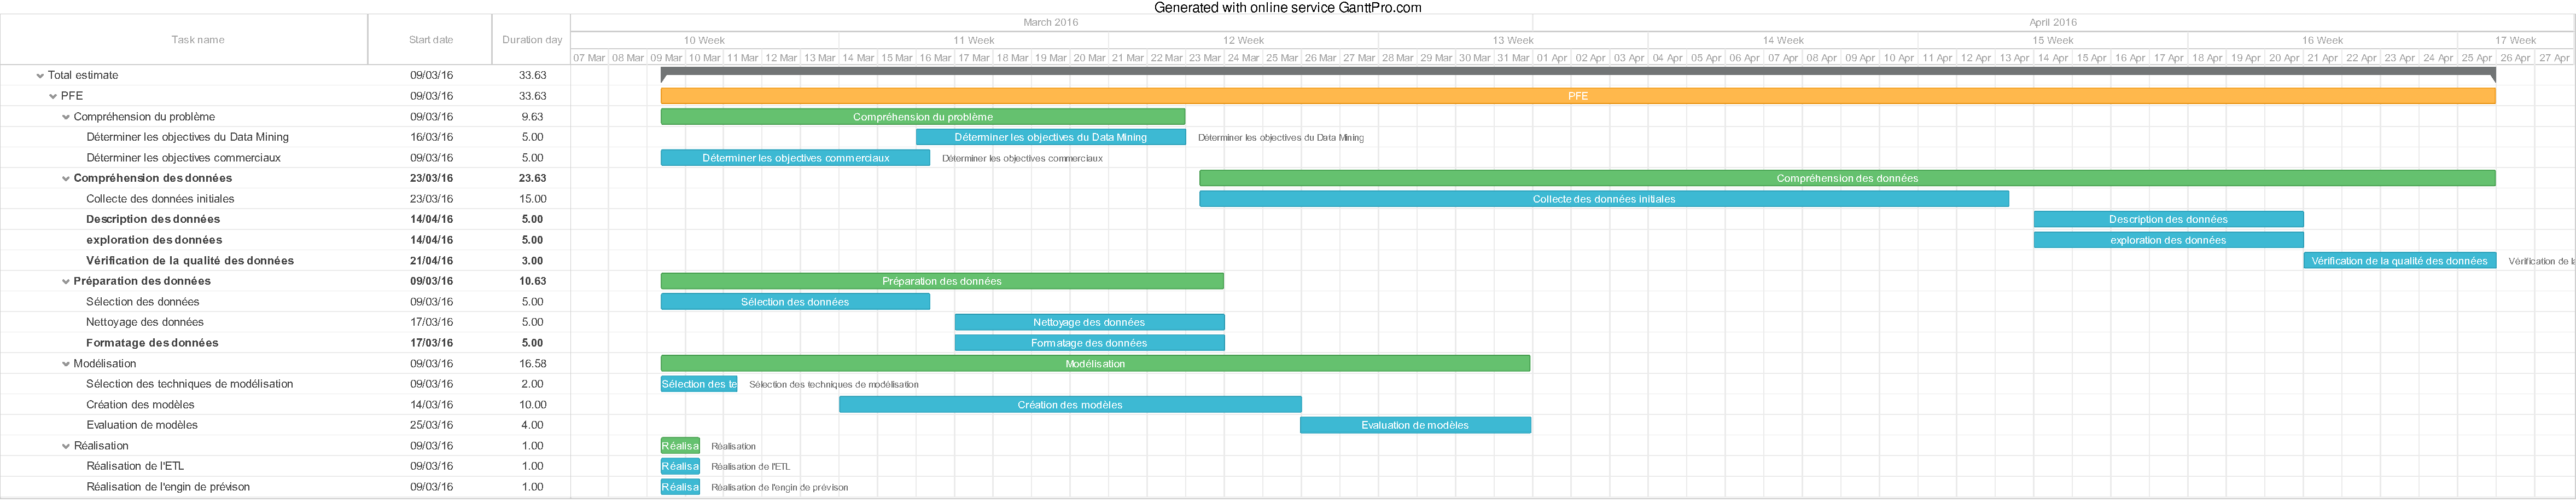
\includegraphics[width=26cm,height=12cm]{gantt.pdf}
    			\caption{Diagramme de GANTT}
    			\label{fig:gantt}
		\end{figure}
	\end{landscape}
	
	\subsubsection{Démarche suivie dans notre projet :}
	Le projet est décomposé en plusieurs lots :
	\begin{description}[align=left]
		\item[Lot I :] Compréhension du problème.
						\begin{itemize}
							\item Comprendre le métier de la cellule Business intelligence de la direction commerciale au sein du groupe OCP.
							\item Détermination des objectives du projet Data Mining.
							\item Détermination des métriques pour l'évaluation de la réussite du projet.
					   	\end{itemize}
		\item[Lot II :] Compréhension des données.
						\begin{itemize}
							\item Description et familiarisation avec les différentes sources de données au sein de l'OCP.
							\item Parsing\footnote{Anglais pour "Analyse syntaxique": processus d'analyse d'une chaîne de symboles soit en langage naturel ou machine suivant les règles d'une grammaire formelle.} des données non structurées concernant les imports et exports des différents produits phosphatés.
							\item Audit de la qualité du résultat du Parsing et analyse préliminaire.
						\end{itemize}		 % Parsing donnees non structure developement ETL + qualites
		\item[Lot III :] Extension des données aux banques externes.
						\begin{itemize}
							\item Recherche et énumeration des différents banques de données Web.
							\item Extraction et formatage des données d'extension.
							\item Jointure et enrichissement des données.
						\end{itemize} %external data world-bank
		\item[Lot IV :] Analyse causale de la demande en engrais.
						\begin{itemize}
							\item L'analyse en composantes principales des différentes données enrichies du lot III.
							\item Sélection des premières composantes principales les plus représentatives.
							\item Regression sur les composantes retenues et interpretation.
						\end{itemize} % analyse causale (ACP + degagement des axes factoriel + Interpretation)
		\item[Lot V :] Analyse en series chronologiques et projections.
						\begin{itemize}
							\item Visualisation exemplaire des séries des demandes de fertilisants.
							\item Etude de la tendance.
							\item Etude de la saisonnalite.
							\item Etude des résidus.
							\item Modélisations SARIMA.
							\item Résultats et conclusions.
						\end{itemize}
		\item[Lot VI :] Réalisation
	\end{description}
